\chapter{非线性积分表达式化简}
\section{引言}\label{Introduction-03}

符号积分是计算机代数的重要组成部分之一. 关于基本初等函数的符号积分的研究开始于符号计算的发展初期. 最早的符号积分软件SAINT\spell{(Symbolic Automated INTegrator)}和SIN\spell{(Symbolic INtegrator)}分别发表于1963年\citep{slagle1963}和1967年\citep{moses1967}. 符号积分中最重要的基础算法是Risch算法\citep{risch1969,risch1970}, 它是近几十年来符号积分发展的基础. 在Risch算法发表后不久, Moses在SIN的改进版本中首次实现了纯超越函数的部分\citep{moses1971}. 而对于基本初等函数的一般情况, 是由Bronstein在1990年首次实现的\citep{bronstein1990}. 几乎所有的计算机代数系统(如 Maple, Mathematica, Axiom, Maxima 和 Reduce), 都是以Risch算法为基础来实现符号积分的计算的. 

当基本初等函数的符号积分被解决以后, 研究者们主要致力于特殊函数的符号积分的研究\citep{cherry1985,cherry1986,bertrand1994,jeffrey1997}. 近年来, 研究者们主要致力于特殊类型的积分, 如相对论库伦积分\citep{paule2012,paule2013}\zdh Feynman积分\citep{blumlein2012,smirnov2015}和参数积分\citep{raab2016}等.

然而, 关于抽象函数的积分的研究却很少. 只有文献\cite{deconinck2009}和文献\cite{poole2010}提出了一个算法来寻找线性可积的抽象函数表达式的积分. 他们的算法主要致力于寻找方程$D_x f=g$的解. 其主要作用是寻找偏微分方程中的守恒定律(conservation law)\citep{poole2011}, 而不是计算一般的抽象函数积分表达式. 但是, 微分方程的求解往往伴随的抽象函数的积分化简. 因此, 本文将抽象函数积分的化简作为一个挑战性的课题进行研究, 并提出一个相应的算法.

在 Maple 和 Mathematica 中, 只有当一个积分表达式的内部可以写成另一个表达式的导数时, 该积分才能被化简. 例如, 
\begin{equation}
\int\!{u_xv+uv_x \dd x}=\int\!{(uv)_x\dd x}=uv.
\label{complete_matched}
\end{equation}
我们称该类积分是\emph{完全匹配的}. 这类积分在其它的文献中也被称为是\emph{可积的}. 此外, Maple 只能化简含单变量抽象函数的积分表达式, 而 Mathematica 能够化简含多变量抽象函数的积分表达式. 

如果积分表达式的内部存在不匹配的项, 我们求称它是\emph{非完全匹配的}. 例如,
\begin{equation}
\int\!{u_xv+2uv_x \dd x}=uv+\int\!{uv_x\dd x}.
\label{incomplete_matched}
\end{equation}
Maple 和 Mathematica 均不能化简上述积分表达式. 

利用 Maple 和 Mathematica 的内置函数可以化简\emph{完全匹配的}线性积分表达式. 但是, 对于积分的多项式, 问题将变得更加复杂. 如果一个多项式能够因式分解为多个线性表达式的乘积, 我们称它是\emph{线性可约的}. 对于这类积分多项式, 可以因式分解之后再用 Maple 和 Mathematica 的内置函数进行积分化简. 例如, 令$a=\int{u_x v \dd x},b=\int{u v_x \dd x},c=uv$, 我们可以得到一个\emph{线性可约的}表达式
\begin{equation}
a^2+2ab+b^2=(a+b)^2=c^2.
\label{liner_reducible}
\end{equation}

但是, 在一般情况下, 多项式并不是\emph{线性可约的}. 例如在和\refeqn{liner_reducible}相同的假设下, 我们有
\begin{equation}
a^2+3ab+b^2=(a+b)^2+ab=c^2+ab.
\label{non_linear_reducible}
\end{equation} 
我们称这种多项式是\emph{线性不可约的}. 目前没有任何算法能够解决这类积分化简问题. 因为这个问题要比因式分解更加困难, 主要是由于这个问题的答案不是唯一的. 也就是说, 我们不能基于 Maple 和 Mathematica 的内置函数来化简这类问题. 

如果考虑嵌套积分的话, 问题将变得更加复杂. 例如, 
\begin{equation}
\int\!{\left(u\cdot\int\!{v_xw\dd x}+u\cdot\int\!{vw_x\dd x}\right)\dd x}=\int\!{uvw\dd x}.
\label{nested_integral}
\end{equation}
Maple 和 Mathematica 都不能化简这样的积分, 因为他们不能自动对积分内部进行自动的因式分解. 有时, 一个嵌套积分需要被看作是一个导数才能完成化简. 例如,
\begin{equation}
\int\!{\left(u\cdot\int\!{v\dd x}+\int\!{u\dd x}\cdot v\right)\dd x}=\int\!{u\dd x}\cdot\int\!{v\dd x}.
\label{integral_as_differential}
\end{equation}
Maple 和 Mathematica 都不能化简这样的积分. 此外, \emph{非完全匹配}和\emph{线性不可约}的表达式可能递归的出现在积分的内部, 这使得化简问题变得越来越困难.

综上所述, 基于 Maple 和 Mathematica 的内置函数, 我们只能化简\emph{线性可约}且\emph{完全匹配}的积分表达式. 而对于更加一般的\emph{线性不可约}且\emph{非完全匹配}的积分表达式, 本文提出了一个算法来解决它们. 本文的算法基于Maple进行实现. 我们将其打包为\texttt{IntSimplify}. 该软件包有两个导出函数: \texttt{IntExpand}用于将输入表达式展开为本文定义的标准形式; \texttt{IntCombine}用于执行积分化简. 

本章的组织结构如下: 在\refsec{Definitions-03}中, 我们将提出一些定义来更好的描述积分化简问题. 在\refsec{Simplify-03}中, 我们将描述本文算法算法的主要框架. 然后, 本文算法的关键细节将在\refsec{Details-03}中进行展开. 接着, 本文将在\refsec{Results-03}中分析本文算法的时间复杂度和化简能力. 最终, 在\refsec{Conclusion-03}中对该算法进行小结.

\section{相关定义}\label{Definitions-03}
\begin{definition}
一个抽象函数的积分表达式(Abstract Integral Expression, 简称 AIE), 是由一些抽象函数(如$u(x,y),v(z,t)$), 在经过下列操作后得到的结果:
\begin{compactenum}[(1) ]
\item 关于自变量的积分;
\item 关于自变量的微分;
\item 上述结果的乘法;
\item 上述结果的线性组合;
\item 上述操作的迭代.
\end{compactenum}
\end{definition}

从而, 我们将AIE定义为一个代数结构. 而一个标准积分表达式(Standard Integral Expression, 简称SIE)则是将AIE展开至积分内部没有加法后的结果. 同时, 我们称SIE中的每一个加法项为标准积分项(Standard Integral Item, 简称SII). 它们的形式化定义如下:
\begin{definition}
设$\mathcal V$是自变量的集合, 而$\mathcal F$是定义在$\mathcal V$上的连续的抽象函数的集合. 对$\mathcal F$中的元素应用乘法\zdh 积分和微分操作之后, 得到的闭集记做$\mathbb F$. 对于任意的$f\in\mathbb{F}$, 我们称其为SII. 即
\begin{equation} 
f =\underbrace{\int\!\int\!\cdots\!\int}_m{ \frac{\partial^n}{\partial v_1 \partial v_2 \cdots \partial v_n} (g_1 g_2 \cdots g_l)\dd u_1 \dd u_2 \cdots \dd u_m}.
\label{int_form}
\end{equation} 
其中, $u_1,\cdots,u_m,v_1,\cdots,v_n \in \mathcal V$. 而$g_1,\cdots,g_l \in \mathcal F$或和$f$具有相同的形式, 即$g_1,\cdots,g_l \in \mathbb F$.
\end{definition}

\begin{definition}
一个SIE是SII的线性组合, 即
\begin{equation}
I = \sum_{k=1}^N{c_k I_k}.
\label{std_form}
\end{equation} 
其中, $c_k \in K$ and $I_k \in \mathbb F$. 
\end{definition}

SIE的定义不仅涵盖了一般的积分和微分表达式, 也涵盖了它们的乘法, 还涵盖了它们的嵌套积分. 由积分的线性性可知, 一个AIE一定能够通过展开加法得到SIE. 我们在\texttt{IntExpand}中实现了该操作. 

基于抽象函数的连续性假设, 我们可以任意交换积分和微分的顺序. 类似地, 乘法也具有交换性. 为了在体现可交换性的同时简化SII的写法, 我们将\refeqn{int_form}重写为
\begin{equation} 
f=\partial^U_V(G). \label{st_form}
\end{equation} 
其中,  $U=[u_1,\cdots,u_m], V=[v_1,\cdots,v_n] \text{~and~} G=[g_1,\cdots,g_l]$ 分别是积分变量\zdh 微分变量和积分项的无序列表. 当$U,V$为空或只含有一个元素时, \refeqn{st_form}在本文中有几个常用的的简写形式:
\begin{equation}
\begin{split}
\partial_x&=\partial^\varnothing_{[x]},  \\
\partial^x&=\partial_\varnothing^{[x]},  \\ 
\partial(G)&=\partial^\varnothing_\varnothing(G).
\end{split}
\end{equation}
最后一个简写是为了区分积分项$\partial(G)$和无序列表$G$. 

从\refeqn{st_form}中可以看出, 一个SII被清晰的划分为三个组成部分. 为了从$f$中反向获取这三个部分, 我们定义了下列操作:
\begin{equation}
IV(f)=U,DV(f)=V,FC(f)=G.
\end{equation}
同时, 如果$f$只含有一个抽象函数, 我们记$TP(f)=simple$, 否则$TP(f)=complex$. 此外, 我们定义$f$的\emph{内部公共因子}
\begin{equation}    
FV(f)=\left\{
\begin{array}{cl}
\bigcap\limits_{g\in FC(f)}{FV(g)}, &\text{if }TP(f)=complex;\\ 
\text{variable set of } f,          &\text{if }TP(f)=simple.
\end{array}
\right.
\end{equation}

将无序列表视为多重集, 就能基于集合的基本操作实现SII的乘法\zdh 积分和微分操作. 即:
\begin{equation}
\begin{split}
\partial(G_1)\cdot\partial(G_2)&=\partial(G_1+G_2),\\
\partial^{U'}_{V'}\partial^{U}_{V}(G)&=\partial^{U+U'}_{V+V'}(G).
\end{split}
\label{ops}
\end{equation}
这里, $+$是并集操作. 递归地应用上述操作可以压缩SII的结构, 使得$TP(f)=complex$蕴含$|FC(f)|\ge 2$. 

基于上述定义, 我们将一个积分多项式表示为SII的线性组合, 且关于SII的乘法\zdh 积分和微分操作能够用多重集的集合操作来实现. 

\section{算法核心框架} \label{Simplify-03}
我们的算法的目标在于将给定的AIE进行等价变换并使其最简. 首先, 本文将在\refsec{all_rules-03}中找到一系列的合并规则. 然后, 在\refsec{optimization-03}找到最优的化简的方案. 事实上, 该化简问题能够表示为一个$\ell_0$-优化问题. 但是因为它是NP-hard的, 我们将求解一个近似的$\ell_1$-优化问题. 


\subsection{寻找所有二项合并规则}\label{all_rules-03}
一般而言, 积分化简中的合并规则有无穷多种不同的形式, 如$u_x v + u v_x = (uv)_x$, $u_x v w+u v_x w + u v w_x = (uvw)_x$等等. 我们不可能一一列举所有情况. 但是, 从另一个角度来看, 所有多于二项的合并规则都能由二项的合并规则导出. 例如, $u_xvw+uv_xw+uvw_x=(uv)_xw+uvw_x=(uvw)_x$. 

对于最简单的二项合并规则$u_x v + u v_x = (uv)_x$, 我们可以对其进行乘法\zdh 积分和微分操作来构造新的合并规则. 忽略合并规则中的常数系数, 我们发现, 所有的二项合并规则都能写成$I_1+I_2=I_3$的形式. 事实上, $I_1,I_2,I_3\in \mathbb F$. 因此, 我们可以基于最简单的二项合并规则获取所有可能的合并规则. 

设一个SIE中的所有SII构成集合$\mathcal I =\{I_1,\cdots,I_N\}$. 设集合$\mathbb I$满足$\mathcal I \subset \mathbb I$, 如果对于任意的$I_1,I_2\in \mathbb I$且$I_1+I_2=I_3$都有$I_3\in \mathbb I$, 我们就$\mathbb I$是$\mathcal I$的\emph{生成集}. 设$\mathbb I=\{B_1,\cdots,B_M\}$, 所有的合并规则就能构成集合$\mathcal R=\{{J_1}_l+{J_2}_l={J_3}_l|{J_1}_l,{J_2}_l,{J_3}_l \in \mathbb I, l=1..L\}$.

构造集合$\mathcal R$的算法如\refalg{FindAllRules}所示. 其中$FindRulesIn(I)$表示在集合$\{(I_1,I_2)|I_1,I_2,\in I\}$中寻找合并规则, 而$FindRulesBetween(I,J)$则表示在集合$\{(I_1,I_2)|I_1\in I, I_2\in J\}$中寻找合并规则. 

\begin{algorithm}
\caption{寻找所有二项合并规则}
\label{FindAllRules}
\KwIn{一个SIE}
\KwOut{所有二项合并规则构成的集合}
\Fn{$FindAllRules(e)$}{
    $I\gets$ set of SIIs in $e$; $R\gets FindRulesIn(I)$\;
    \While{$\bf{true}$}{
        $J\gets$ new SIIs in $R$\;
        \lIf{$J=\emptyset$}{$\bf{break}$}
        $R\gets R \cup FindRulesIn(I) \cup FindRulesBetween(I,J)$\;
    }
    \Return{$R$}\;
}
\end{algorithm}

\refalg{FindAllRules}的时间复杂度直接决定了本文积分化简算法的复杂度. 该算法的复杂度取决于生成集$\mathbb I$中的元素个数. 记生成集的元素个数为$N$, 则该算法的复杂度是$\mathcal O(N^2)$. 尽管$N$的大小无法根据输入表达式直接确定, 但是可以估计到它的最差情况. 考虑
\begin{equation}
I_n=\int\!{(f_1\cdot f_2\cdots f_n)_x \dd x},
\label{worst_case}
\end{equation}
其中$f_1,f_2,\cdots,f_n$是互不相同的抽象函数. \refeqn{worst_case}在展开后有$n$个积分项, 这些项构成了集合$\mathcal I$. 集合$\mathcal I$的任一非空子集中的项都能够合并, 合并后都能生成$\mathbb I$中一个不同的项. 因此, $N=2^n-1$. 所以\refalg{FindAllRules}的时间复杂度为$\mathcal O(4^n)$. 从而, 我们可以将输入表达式中含不同函数最多的乘法项中函数的个数定义为改输入表达式的阶数. 于是, 该算法关于输入表达式的阶数的时间复杂度是指数的. 

\subsection{化简对应的优化问题}\label{optimization-03}
一旦建立了集合$\mathcal R$, 化简问题就能表示为一个等价变换
\begin{equation}
I=\sum_{k=1}^N{c_k I_k}-\sum_{l=1}^L{x_l ({J_1}_l+{J_2}_l-{J_3}_l)},
\label{normal_simplify}
\end{equation}
其中${J_1}_l+{J_2}_l={J_3}_l(l=1..L)$是集合$\mathcal R$中的元素. 然后, 化简问题就能转化为选择最优$x_l(l=1..L)$的优化问题.

一般情况下, 化简是为了最小化项数或最简化系数. 为了更好的表达这两个目标, 我们可以将\refeqn{normal_simplify}转化为成矩阵形式. 

设 
\begin{equation}
\begin{split}
\sum_{k=1}^N{c_k I_k} &= \sum_{k=1}^M{b_k B_k},\\
\sum_{l=1}^L{x_l ({J_1}_l+{J_2}_l-{J_3}_l)} &= \sum_{j=1}^L{x_j \sum_{i=1}^M{a_{ij} B_i}}.
\end{split}
\end{equation} 
令$\bm B=(B_1,\cdots,B_M),\bm b=(b_1,\cdots,b_M)\TT,\bm x=(x_1,\cdots,x_L)\TT,\bm A=(a_{ij})_{M \times L}$, \refeqn{normal_simplify}可以写成 
\begin{equation}
I=\bm{B}\bm{b}-\bm{B}\bm{A}\bm{x}=\bm{B}(\bm{b}-\bm{A}\bm{x}).
\end{equation}

为了最小化项数, 我们需要做一个$\ell_0$-优化
\begin{equation}
    \underset{\bm x}\min~\VecNorm{\bm{b}-\bm{A}\bm{x}}_0,
\end{equation}
其中$\VecNorm{\bm x}_0$是$\ell_0$-范数. 因为这个问题是NP-hard的, 我们可以求解另一个相对简单的近似优化问题
\begin{equation}
\underset{\bm x}\min\VecNorm{\bm{b}-\bm{A}\bm{x}}_1.
\label{LAE}
\end{equation}
在这个问题中, 我们不仅能够近似地最小化项数, 还能最简化系数. 

事实上, $\ell_1$-优化能够转化为一个线性规划\citep[pp. 195--196]{L1_regression}, 即
\begin{equation}
\begin{split}
&\underset{\bm u,\bm x}\min \sum_{k=1}^L{u_k},\\
&s.t. \left\{
\begin{matrix}
\bm{u}\ge \bm{b}-\bm{A}\bm{x},\\ 
\bm{u}\ge \bm{A}\bm{x}-\bm{b},
\end{matrix}
\right.
\end{split}
\label{LP}
\end{equation}
其中 $\bm u=(u_1,\cdots,u_L)\TT$. 这些约束条件能够使得问题求得最优解时满足$\bm u = |\bm{b}-\bm{A}\bm{x}|$. 所以, 该优化问题和原问题是等价的. 同时, 该问题又不包含绝对值操作, 因此它能够被线性规划算法求解. 

最终, 我们将积分化简的问题转换为一个线性规划问题进行求解.

\section{关键的子算法} \label{Details-03}
In this section, the details of finding combination rules would be expounded in \refsec{Combine-03}, and the details of optimization methods would be described in \refsec{optMethods-03}.

\subsection{Algorithm of finding combination rules} \label{Combine-03}

All possible combination rules can be found based on the algorithm of finding combination rules between two different SIIs. The details of this algorithm will be described in this section. 

For the simplest combination rule $u_x v + u v_x = (uv)_x$, we can do multiplication, integral and  differential on it to construct new rules. Hence, for any combinable pair, the combination rule can be reduced to the simplest form that contains only two abstract functions. 

Assume that $I_1,I_2$ are SIIs, consider the combination 
\begin{equation}
\begin{split}
I_1+I_2 &= \partial^U_V(j_1) + \partial^U_V(j_2) \\
        &= \partial^U_V( j_1+j_2 )\\
        &= \partial^U_V( f\cdot(j_3+j_4) )\\ 
        &= \partial^U_V( f\cdot r ) = I_3 .
\end{split}
\label{combine_form}
\end{equation} 

The second equality holds when $I_1,I_2$ have the same integral and differential variables, i.e., $IV(I_1)=IV(I_2),DV(I_1)=DV(I_2)$. The common part between $j_1$ and $j_2$ is extracted and denoted as $f$ in the third equality, and the rest parts are denoted as $j_3,j_4$, respectively.

If the third equality holds outside an integral, it represents the situations like 
\begin{equation}
f\cdot\int\!{u_x v\dd x}+f\cdot\int\!{u v_x \dd x} = f\cdot(uv).
\end{equation} 
Since $f$ is arbitrary, when taking $f=1$, it represents the combination of linear cases; when taking $f$ as a multiplication of integrals, it represents the combination of polynomials. It means that our algorithm is capable of processing polynomial of integrals. 

If the third equality holds inside an integral, it represents the situations like 
\begin{equation}
\int\!{f \left(\int\!{u_x v\dd x}\right)\dd y}+\int\!{f \left(\int\!{u v_x \dd x}\right) \dd y} = \int\!{fuv\dd y}.
\end{equation}
It means that our algorithm also works well for nested integrals. 

The last combination in \refeqn{combine_form} that $j_3+j_4=r$ can be considered by two cases: \emph{root case} and \emph{recursive case}. 

The \emph{root case} means that $j_3+j_4$ can be combined by the most basic differential rule with two items, i.e., 
\begin{equation}
\begin{array}{rl}
& j_3+j_4=u \cdot v+\partial^x(u)\cdot \partial_x(v) = \partial^x(u)\cdot v, \\
\text{or}& j_3+j_4=u \cdot v+\partial_x(u)\cdot \partial^x(v) = \partial^x(v)\cdot u.
\end{array}
\label{root_form}
\end{equation}

The \emph{recursive case} means that $j_3+j_4$ can be combined  finally by using  \refeqn{combine_form} recursively. It implies that $j_3,j_4$ are integrals, not the multiplication of integrals.

For these two cases, it is required that the inner part of integrals is finally multiplied by two parts. So it requires $TP(I_1)=TP(I_2)=complex$.  

Based on the above analysis, we introduce the Algorithm \ref{FindRuleForPair}. For the input pair $I_1,I_2$, we check the common conditions of \emph{root case} and \emph{recursive case}. Then, we fetch $J_1,J_2$ as the inner parts of $I_1,I_2$, respectively. After that, we use set operations to compute the common part of $J_1$ and $J_2$, and denote the different parts of $J_1,J_2$ as $J_3,J_4$, respectively. Finally, we try to combine $J_3,J_4$ directly. If it fails and $|J_3|=|J_4|=1$, we would try to combine them recursively.  

\begin{algorithm}
\caption{Finding combination rules for two integral items.}
\label{FindRuleForPair}
\KwIn{IntFunc object $I_1,I_2$, external integral variables  $S$.}
\KwOut{Return $I_3$ if $I_1 + I_2 = I_3$, or $FAIL$ if $I_1,I_2$ cannot be combined.}
\Fn{$FindRuleForPair(I_1,I_2,S)$}{
    \tcp{Check the common condition.}
    \lIf{\bf{not} $( TP(I_1)=TP(I_2)=complex$  \bf{and} $IV(I_1)=IV(I_2)$ \bf{and} $DV(I_1)=DV(I_2) )$}{
        \Return{$FAIL$}
    }
    \tcp{Initialization}
    $U \gets IV(I_1), V\gets DV(I_1),S\gets U \cup S $\;
    $J_1\gets FC(I_1), J_2\gets FC(I_2) $ \;
    $F\gets J_1 \cap J_2, J_3\gets J_1-F, J_4\gets J_2-F$\;
    \tcp{Ensure $|J_3|\le |J_4|$}
    \lIf{$|J_3|>|J_4|$}{
        $J_3,J_4\gets J_4,J_3$
    }
    \tcp{Try combine directly.}
    \uIf{$\min(|J_3|,|J_4|)=1$}{
        $r,F\gets FindRuleForVars1(\partial(J_3),\partial(J_4),F,S)$\;
    }\uElseIf{$\min(|J_3|,|J_4|)=2$}{
        $r\gets FindRuleForVars2(\partial(J_3),\partial(J_4),S)$\;
    }\lElse{
        $r\gets FAIL$
    }
    \tcp{Try combine recursively.}
    \If{$r=FAIL$ \bf{and} $|J_3|=|J_4|=1$}{
        $r\gets FindRuleForPair(\partial(J_3),\partial(J_4),S) $\;
    }
    \tcp{Build rule.}
    \lIf{$r\neq FAIL$}{
        \Return{$\partial^U_V(\partial(F)\cdot r)$}
    }
    \Return{$FAIL$}\;
}
\end{algorithm}

\begin{algorithm}
\caption{Finding combination rules for normal root cases.}
\label{FindRuleForVars2}
\Fn{$FindRuleForVars2(I_1,I_2,S)$}{
    $[u,v]\gets FC(I_1)$\tcp*[l]{Extract contents of multiset.}
    \For{$x\in S\cap FV(I_1) \cap FV(I_2)$}{
        \lIf{$\partial_x(u) \cdot \partial^x(v)=I_2$}{
            \Return{$\partial_x(u \cdot \partial^x(v) )$}
        }
        \lElseIf{$\partial^x(u) \cdot \partial_x(v)=I_2$}{
            \Return{$\partial_x(\partial^x(u) \cdot v )$}
        }
    }
    \Return{$FAIL$}\;
}
\end{algorithm}

\begin{algorithm}
\caption{Finding combination rules for special root cases.}
\label{FindRuleForVars1}
\Fn{$FindRuleForVars1(u,t,F,S)$}{
    \lIf{$TP(u)\neq complex$}{
        \Return{$FAIL,F$}
    }
    $G \gets FC(u) \cap F$\;
    \For{$v \in G$}{
        $I_1\gets u \cdot v,I_2 \gets t\cdot v$\;
        \For{$x \in S\cap FV(I_1) \cap FV(I_2)$}{
            \uIf{$\partial_x(u) \cdot \partial^x(v)=I_2$}{
                $F\gets F-[v]$\;
                \Return{$\partial_x(u \cdot \partial^x(v) ),F$}\;
            }
            \ElseIf{$\partial^x(u) \cdot \partial_x(v)=I_2$}{
                $F\gets F-[v]$\;
                \Return{$\partial_x(\partial^x(u) \cdot v ),F$}\;
            }
        }
    }
    \Return{$FAIL,F$}\;
}
\end{algorithm}

There are three major differences between the above mathematical description and the algorithmic description in the pseudo-code. 

Firstly, we use multisets instead of SIIs to perform calculations. The symbols of multisets are capitals of integral items. 

Secondly, the \emph{root case} is divided into two sub cases due to the flexibility of collection. 

For the normal case $|J_3|=|J_4|=2$, we can test the two possibilities directly as  \refeqn{root_form}. Sometimes, 
\begin{equation}
j_1+j_2 = f \cdot ( u \cdot (v_1 \cdots v_n)_x +  u_x \cdot (v_1 \cdots v_n ) ).
\end{equation}
Therefore, $|J_3|=2,|J_4|=n+1\ge 2$. Such cases can be handled by the same procedure as the normal case, so they can be grouped together under the condition $\min(|J_3|,|J_4|)=2$. Such cases can be processed by Algorithm \ref{FindRuleForVars2}.

For the special case, there might be 
\begin{equation}
\begin{split}
j_1 + j_2   &= f \cdot ( j_3 g + j_4 g ) \\ 
            &= f \cdot ( (g \cdot t_1\cdots t_n)_x\cdot g + (g \cdot t_1\cdots t_n)\cdot g_x ),
\end{split}
\end{equation}
where $j_3=(g \cdot t_1\cdots t_n)_x , j_4=t_1\cdots t_n\cdot g_x$ with $\min(|J_3|,|J_4|)=1$. In such case, we have $TP(j_3)=complex, g\in FC(j_3)\cap F$. So we can try every possible $g$ to find combination rules as described in Algorithm \ref{FindRuleForVars1}. 

Finally, there is an external parameter $S$ in the pseudo-code. It means that there are some external integral operations outside the current recursion. As we know, if there is no integral operation, such as $u_x v + u v_x = (uv)_x$, a combination would be restored after expansion. By default, we only combine the integrals like $\int\!{u_x v\dd x} + \int\!{u v_x\dd x} = uv$ by taking $S=\varnothing$. But if we want to perform the previous combination, we can set $S$ to be the whole variable set $\mathcal V$. 
% As described in \refsec{implementation-03}, this behavior is controlled by the parameter \texttt{CombineDiff}.

In the Algorithms \ref{FindRuleForVars2} and \ref{FindRuleForVars1}, we only search the differential rules about variables in the set $S$.  The basic rule $u_x v + u v_x = (uv)_x$ holds when $x$ is the independent variable of $u$ and $v$. So, we would reduce $S$ to the intersection of $FV(I_1),FV(I_2)$ and $S$, which is shown in the pseudo-code.

In short, we have explained the details of finding combination rules between two integral items. Here is a typical example for this algorithm. Let 
\begin{equation}
a=\int\!{uu_xv \dd x},~~b=\int\!{u^2v_x\dd x},~~c=\int\!{u(uv)_x\dd x},~~d=u^2v.
\end{equation}
We have the linear combination rules $\{a+b=c,a+c=d\}$. 

For $a+b=c$, we have $F=[u],J_3=[u_x,v],J_4=[u,v_x]$, which can be handled by the Algorithm \ref{FindRuleForVars2}.

For $a+c=d$, we have $F=[u],J_3=[(uv)_x],J_4=[u_x,v]$, which can be processed by the Algorithm \ref{FindRuleForVars1}.  

For the \emph{incomplete matched} expression $3a+b$,
we can get the optimized result $a+d$ by solving the corresponding optimization problem.

For polynomial $5a^2+4ab+b^2$, which is \emph{linear unreducible}, we would get the following 8 rules with 10 SIIs by the \emph{recursive cases} based on the Algorithm \ref{FindAllRules}, i.e., 
\begin{equation}
\left\{ 
\begin{matrix}
a^2+ab=ac, &ab+b^2=bc, &ac+bc=c^2, \\
ad+bd=cd,  &a^2+ac=ad, &ab+bc=bd,  \\ 
ac+c^2=cd, &ad+cd=d^2. &
\end{matrix}
\right\}
\end{equation}
As an example of these rules, for $a^2+ab=ac$, we would have $F=[a],J_3=[a],J_4=[b]$ for the first level of recursion, then get $a+b=c$ in the second level of recursion. Finally, we can get the best result $a^2+d^2$ by solving the related optimization problem. 

\subsection{Discussion of optimization methods}\label{optMethods-03}

As described in \refsec{optimization-03}, the simplification problem is equivalent to a linear programming (LP) problem. But, our problem cannot be solved by numerical LP algorithms directly. Once existing numerical errors, there would be a lot of superfluous rest items with tiny coefficients. It is difficult to determine whether these items actually exist or caused by numerical errors. Thus, we need to do exact linear programming (ELP) in our problem. 

There are some ELP implementations, such as \texttt{simplex} in Maple, \texttt{LinearProgramming} in Mathematica, \spell{SoPlex} \citep{soplex} and \spell{Qsopt-ex} \citep{qsoptex}. Since most ELP implementations aim to solve the problem on rational field, we should transform our problem into it. 

Review the definition of SIE in \refeqn{std_form}, we assume the coefficients $c_k\in K$, and the SIIs $I_k\in \mathbb F$. The simplification problem is dependent on these two sets, we use $K[\mathbb F]$ to denote it. In general, we should solve $\mathbb C[\mathbb F]$. Regard the imaginary unit $i$ as a constant, $\mathbb C[\mathbb F]=\mathbb R[\mathbb F \cup \{i\}]$. Furthermore, regard all  irrational numbers as constants, we have $\mathbb C[\mathbb F]=\mathbb Q[F\cup (\mathbb R - \mathbb Q) \cup \{i\}]$. Finally, we can solve the ELP on rational field.

For example, consider
\begin{equation}
\left(1+\sqrt{2}\right)\ii{u_x v}+\sqrt{2}\ii{u v_x}, 
\end{equation}
we have
\begin{equation}
\bm{B}=\left(
\begin{array}{c}
\ii{u_x v}  \\
\ii{u v_x}  \\
u v         \\
\sqrt{2}\ii{u_x v}  \\
\sqrt{2}\ii{u v_x}  \\
\sqrt{2}u v         \\
\end{array}
\right)\TT,
\bm{b}=\left(
\begin{array}{c}
1   \\
0   \\
0   \\
1   \\
1   \\
0   \\
\end{array}
\right),
\bm{A}=\left(
\begin{array}{rr}
1   & 0\\
1   & 0\\
-1  & 0\\
0   & 1\\
0   & 1\\
0   & -1\\
\end{array}
\right).
\end{equation}
Solve the related ELP, the optimal solution is $\bm{x}=\left(0,1\right)\TT$, and the simplified result is $\sqrt{2}uv+\ii{u_x v}$. 

There is another way to avoid numerical errors. We can do numerical integer linear programming (NILP) instead of ELP, and round the result to integers. In theory, ILP is more difficult than LP, because ILP is NP-hard. But, numerical algorithms is faster than symbolic algorithms in practice. So, NILP algorithms maybe faster than ELP algorithms in some cases.

Based on the considerations above, we have integrated several optimization algorithms in our program:
\begin{compactitem}[\textbullet]
\item \texttt{SLP}, which means \texttt{simplex} in Maple, is a ELP algorithm; 
\item \texttt{mmaSLP}, which means \texttt{LinearProgramming} in Mathematica, is a ELP algorithm;
\item \texttt{SoPlex} \citep{soplex} is a ELP algorithm that implemented in C++;
\item \texttt{NILP}, which means \texttt{LPSolve} in Maple, is a NILP algorithm;
\item \texttt{MatlabILP}, which means \texttt{intlinprog} in Matlab, is a NILP algorithm.
\end{compactitem}

Now, a concrete example is given to compare their running time for different scales. Let $\mathcal F=\{f_1,f_2,\cdots\}$, consider the expression
\begin{equation}
\left(\sum\limits_{k=1}^{n_1}{\int\!{(f_{i_{2k-1}}f_{i_{2k}})_x\dd x}}\right)^2+\sum\limits_{k=1}^{n_2}{\int\!{(f_{j_{3k-2}}f_{j_{3k-1}}f_{j_{3k}})_x\dd x}},
\end{equation}
where $i_k,j_k \in \{1,2,\cdots\}$. In order to control the number of generated items, we take $n_1\le 8,n_2\le 8$ in the experiment. The runtime of solving optimization problems by different algorithms is shown in \reffig{opts_log}. For a clearer comparison of them, we take the logarithm of runtime.

\begin{figure}[htb]
\centering
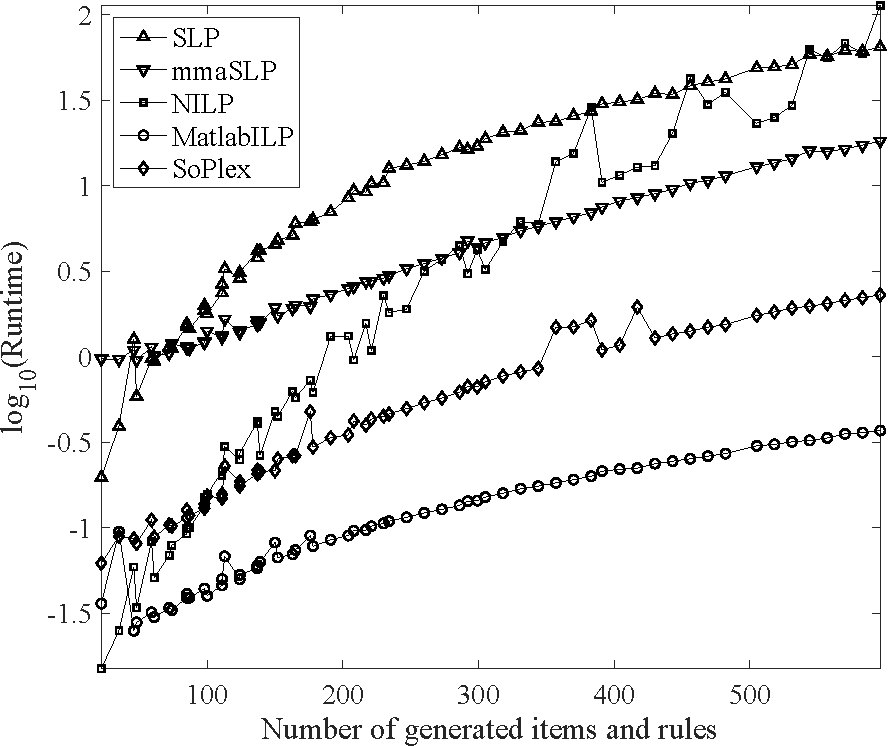
\includegraphics[width=0.8\textwidth]{fig/int-6.pdf}
\caption{Log scaled runtime about optimization methods}\label{opts_log}
\label{opts_all}
\end{figure}

It can be seen from \reffig{opts_all}, the growth trend of runtime of ELP algorithms are similar. But \texttt{SoPlex} is much faster than the others. The runtime of \texttt{SoPlex} did not exceed 2 seconds in our tests.

Although ILP is much harder than LP, the advantage of numerical calculation makes numerical ILP algorithms faster than symbolic LP algorithms. For example, \texttt{NILP} is faster than \texttt{SLP} and \texttt{mmaSLP} when the scale of problem is less than 250. The further developed NILP algorithm \texttt{MatlabILP} is significantly faster than \texttt{SLP} and \texttt{mmaSLP} within our experiments. 

In addition, we can't say that \texttt{MatlabILP} is faster than \texttt{SoPlex}. Because we invoke \texttt{SoPlex} through command line interface, which spend much time in file IO and program launching.

In conclusion, \texttt{SoPlex} and \texttt{MatlabILP} are the most efficient optimization algorithms in our problem.

\section{Experiments} \label{Results-03}
In this section, we will compare our algorithm with those existing ones in \refsec{sec5.1-03}, and analyze the time complexity of our algorithm in \refsec{sec5.2-03}.

\subsection{Comparison of capability of simplification}\label{sec5.1-03}
In order to compare our algorithm with those existing ones in Maple and Mathematica in detail,  we introduce the following 7 criterions to classify integrals:
\begin{compactenum}[1) ]
\item The number of multiplied functions inside an integral is more than 2.
\item The expression contains incomplete matched integrals.
\item Some nested integrals should be regarded as differentials.
\item The nested integrals can be simplified recursively. 
\item The polynomial of integrals is linear unreducible.
\item The abstract function is composite with nonlinear functions, such as $u^{-1}$, $\sin(u)$, etc.  
\item The expression contains specific functions such as $x$, $\sin(x)$, etc. 
\end{compactenum} 
These 7 criterions divide all integrals into 128 classes. The classification of an integral can be represented by a binary sequence with the length 7, where 1 represents true and 0 represents false. The increase in the number of 1 in a binary sequence means a more general situation.

As shown in Table \ref{tb1}, based on the control variate method, we choose 10 different classes of integral to show the effectiveness of each criterion. For each case, we construct a typical integral for testing. Limited by the table width, we use a simplified notation to represent integrals. For example, $\int\!{(uv)_x\dd x}=\int\!{u_xv\dd x}+\int\!{uv_x\dd x}$. The differential inside an integral will be expanded, not eliminated. The first column indicates the classification of the expression. The binary sequence in the second column means the capability of Maple, Mathematica and our algorithm successively. The testing code of Maple is \texttt{eval(factor(combine(e)))}. The testing code of Mathematica is 
\begin{verbatim}
Factor[e//.{
    p_?NumericQ*Integrate[a_,c_]+Integrate[b_,c_]
    :>Integrate[p*a+b,c],
    Integrate[a_,c_]+Integrate[b_,c_]
    :>Integrate[a+b,c],
    p_?NumericQ*Integrate[a_,c_]
    +q_?NumericQ*Integrate[b_,c_]
    :>Integrate[p*a+q*b,c]
}];
\end{verbatim}

% 1. 二项、多项
% 2. 完全匹配,不完全匹配
% 3. 无积分,积分作为导数
% 4. 无递归积分,有递归积分
% 5. 是否线性可约
% 6. 有无复合
% 7. 有无混合
\begin{table}[htb]
\renewcommand{\arraystretch}{1.25}
\centering
\caption{Comparison of capability of simplification} \label{tb1}
\renewcommand{\dd}[1]{\mathrm{d}#1}
\renewcommand{\ii}[1]{\int\!{#1\dd x}}
\begin{tabular}{ccl}
\hline
Type & Result & \multicolumn{1}{c}{Expression} \\
\hline
0000000 & 111 & $I_1=\int\!{(uv)_x\dd x}$\\ 
1000000 & 111 & $I_2=\int\!{(u^2v)_x\dd x}$\\ 
0100000 & 001 & $I_3=I_1+\int\!{u_xv\dd x}$\\ 
0010000 & 001 & $I_4=\int\!{(\int\!{u\dd x}\cdot \int\!{v\dd x})_x\dd x}$\\
0001000 & 001 & $I_5=\int\!{u\cdot \int\!{(vw)_x\dd x}\dd x}$\\
0000100 & 001 & $I_6=I_1^2+\int\!{(vw)_x\dd x}$\\
0000010 & 100 & $I_7=\int\!{(\sin(u)\sqrt{v})_x\dd x}$\\
0000001 & 110 & $I_8=\int\!{(\sin(x)u)_x\dd x}$\\
1111100 & 001 & $I_9=\int\!{(\int\!{u\dd x}\int\!{(\int\!{uv\dd x}\;w)_x\dd x\dd x})_x\dd x}+I_3^2$\\
1111111 & 000 & $I_{10}=I_9+\int\!{(\sin(x)/u)_x\dd x}$\\
\hline
\end{tabular}
\end{table} 

As we can see from Table \ref{tb1}, Maple and Mathematica can only process linear reducible polynomials of simple integrals. They require that the inside of integrals should be complete matched and do not contain nested integrals. In addition, Mathematica may fail to simplify some complete matched integrals. However, our proposed algorithm \texttt{IntCombine} can handle arbitrary polynomials of complex integrals. The inside of an integral can be incomplete matched and even contain nested integrals. From $I_7$ and $I_8$ we know, \texttt{IntCombine} do not support expressions containing specific or composite functions, but Maple and Mathematica can process simple cases of them. However,  \texttt{IntCombine} can process all other cases according to $I_9$. The most general case $I_{10}$ cannot be handled by any algorithm mentioned in Table \ref{tb1}. 

To further show the effectiveness of \texttt{IntCombine}, a more complicated example that contains 50 items is considered, i.e.,
\begin{equation}
\def\arraystretch{1.5}
\begin{array}{l}
-20u_xw_{xx}v
+c\ii{u_{xxxxx}\ii{v}}
+c\ii{u_{xxxxx}v}
+c\ii{v_{xxxxx}u}\\% 1
+20u_x^2v_xa
+20u_x\ii{wv_{xxx}}
+20w_x\ii{v_xu_{xx}}
+20w_x\ii{u_xv_{xx}}\\% 2
+10c\ii{v_{xxx}u^2}
+30c\ii{uu_xv_{xx}}
-20u_xwv_{xx}
-60cuu_x\ii{uv}\\% 3
+10c\ii{u_x\ii{u_xv_{xx}}}
+10c\ii{u_x\ii{v_xu_{xx}}}
-30vu^3c
-40u_xw_xv_x\\% 4
+30c\ii{u^2u_{xx}\ii{v}}
+20c\ii{v_xu_{xx}u}
+30c\ii{u_{xxx}u_x\ii{v}}\\% 5
+30c\ii{u_{xx}vu_x}
+40u_x\ii{w_xv_{xx}}
+40u_x\ii{v_xw_{xx}}
-120uu_xwv\\% 6
-4u_x^2v_xb
+20u_x\ii{vw_{xxx}}
+120u_x\ii{vuw_x}
+120u_x\ii{uvw_x}\\% 7
+60c\ii{uu_x^2\ii{v}}
+120c\ii{u^2u_xv}
-cuv_{xxxx}
-10u_{xxx}c\ii{vu}\\% 8
-10u_{xxx}c\ii{u_x\ii{v}}
-20u_xa\ii{u_xv_{xx}}
-20u_xa\ii{v_xu_{xx}}\\% 9
+4u_xb\ii{u_xv_{xx}}
-10cu\ii{u_xv_{xx}}
-10c v u u_{xx}
-10cu\ii{v_xu_{xx}}\\% 10
+4u_xb\ii{v_xu_xx}
+20c\ii{u_{xx}^2\ii{v}}
-cu_{xxxxx}\ii{v}\\% 11
+10c\ii{u_{xxxx}u\ii{v}}
+30u^2u_xc\ii{v}
-60uu_xc\ii{u_x\ii{v}}\\% 12
-20cu_xu_{xx}\ii{v}
+120u_x\ii{vwu_x}
+c\ii{u_xv_{xxxx}}
-10v_{xx}u^2c\\% 13
+30c\ii{u^3v_x}
+20c\ii{vu_{xxx}u},\\% 14
\end{array}
\label{big50}
\end{equation}
where $u=u(x,t),v=v(x,t),w=w(x,t)$, and $a,b,c$ are constants. 

Our algorithm can simplify it within 4 seconds, the obtained result is 0. There are a lot of complicated combination rules used in this example. Due to the space limitations, we only show two of them here. Firstly, we have 
\begin{equation}
\def\arraystretch{1.5}
\begin{array}{l}
0=u_x\int\!{v_{xx}w_x\dd x}+u_x\int\!{v_xw_{xx}\dd x}-u_xv_xw_x\\
~~+w_x\int\!{u_xv_{xx}\dd x}+w_x\int\!{u_{xx}v_x\dd x}-u_xv_xw_x\\
~~+u_x\int\!{vw_{xxx}\dd x}+u_x\int\!{v_xw_{xx}\dd x}-u_xvw_{xx}\\
~~+u_x\int\!{v_{xxx}w\dd x}+u_x\int\!{v_{xx}w_x\dd x}-u_xv_{xx}w.
\end{array}
\label{counter_example}
\end{equation}
Here, $u_x\int\!{v_{xx}w_x\dd x},u_x\int\!{v_xw_{xx}\dd x}$ and $u_xv_xw_x$ are appropriately distributed to four different combinations, which needs some human intelligence but can be done automatically by \texttt{IntCombine}. It is a good example to show why we cost so much time to find all combination rules rather than to simplify the expression step by step. Because the rest six items will not be combined if we eliminate these three items first. 

Secondly, we have 
\begin{equation}
\def\arraystretch{1.5}
\begin{array}{l}
c\int\!{\int\!{v\dd x}uu_{xxxx}\dd x}+c\int\!{\int\!{v\dd x}u_xu_{xxx}\dd x}=c\int\!{\int\!{v\dd x}(uu_{xxx})_x\dd x},\\
c\int\!{\int\!{v\dd x}(uu_{xxx})_x\dd x}+c\int\!{vuu_{xxx}\dd x}=cuu_{xxx}\int\!{v\dd x}.
\end{array}
\end{equation} 
The diversity of nested integrals like this shows another advantage of our algorithm. 

\subsection{Analyzing the time complexity}\label{sec5.2-03}
In this section, we will analyze the time complexity of our algorithm in practice.

In order to test time cost of the worst cases in practice, we take $n$ in \refeqn{worst_case} from 2 to 8, and get the results as shown in \reffig{order}. It can be seen that the time cost grows exponentially. Roughly, the runtime times 4 as the order increases 1, which is consistent with the theoretical analysis in \refsec{all_rules-03}. 

\begin{figure}[htb]
\centering
\subfigure{
    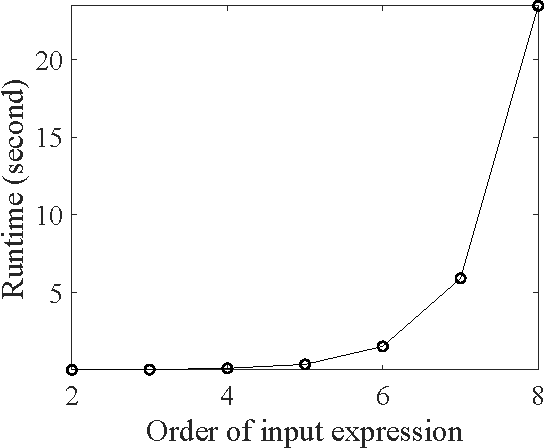
\includegraphics[width=0.45\textwidth]{fig/int-1.pdf}
    \label{order}
}
\subfigure{
    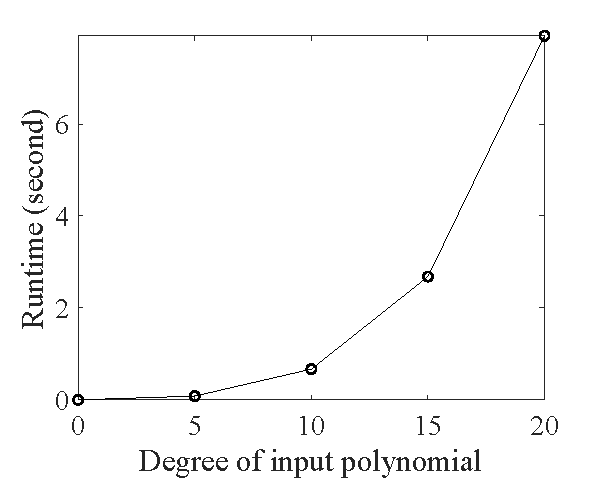
\includegraphics[width=0.45\textwidth]{fig/int-2.pdf}
    \label{degree}
}
\caption{(a) Runtime about order; (b) Runtime about degree}
\end{figure}

It seems that our algorithm is terrible in complexity. However, in practice, there are few cases that more than eight different functions are multiplied in an expression.

In fact, consider the polynomial 
\begin{equation}
\left(\int\!{(f_1\cdots f_n)_x\dd x}\right)^m,
\label{poly}
\end{equation}
where $f_1,\cdots,f_n$ are different functions. The inner part has $M=2^n-1$ items in our algorithm. The number of  monomials generated by them is $\binom{m+M-1}{m}$, where $\binom{A}{B}$ represents binomial coefficient. Thus, the complexity is 
\begin{equation}
\mathcal O\left(\binom{m+2^n-2}{m}^2\right).
\label{polynomial_complexity}    
\end{equation}
For large $n$, it is still exponential. However, for limited $n$, it is equivalent to $\mathcal O(m^{2N})$, where $N=2^n-2$. In other words, the complexity is polynomial, which is acceptable in practice. 

We take $n=2,m\le 20$ in \refeqn{poly}, the runtime of these expressions are shown in \reffig{degree}. For polynomial whose degree is more than 20, our program can solve it within 8 seconds. 

Our algorithm will be more efficient for lower order and lower degree expressions, even for expressions with a large number of input items. For such inputs, there are two techniques to  accelerate the calculation.

The first technique is to keep a remember table. In general, different integral items might contain the same components, so the combine rules of \emph{root cases} might be the same. For example, as mentioned in the end of \refsec{Combine-03}, rules like $ad+bd=cd$ and $ac+bc=c^2$ will be reduced to the same root rule $a+b=c$. It can be accelerated if we remember all rules have been used. It can be implemented easily in Maple by taking advantage of the \verb|option remember| \citep{maple_programming}. 

The second technique is to group the input expression. We notice that two SIIs only can be combined if they have the same $FR$, where
\begin{equation}    
FR(f)=\left\{
\begin{array}{cl}
\prod\limits_{g\in FC(f)}{FR(g)}, &\text{if }TP(f)=complex,\\ 
f,           &\text{if }TP(f)=simple.
\end{array}
\right.
\end{equation} 
Thus, we can use this to accelerate calculation. 

According to \refeqn{polynomial_complexity}, for limited orders and degrees, the time cost of a group would be a limited constant, so the complexity would be linear about the number of input items.  

Let $\mathcal F=\{f_1,f_2,\cdots,f_n\}$, consider the expression
\begin{equation}
\left(\sum\limits_{k=1}^{n_1}{\int\!{(f_{i_{2k-1}}f_{i_{2k}})_x\dd x}}\right)^4+\left(\sum\limits_{k=1}^{n_2}{\int\!{(f_{j_{3k-2}}f_{j_{3k-1}}f_{j_{3k}})_x\dd x}}\right)^2,
\label{construct}
\end{equation}
where $i_k,j_k \in \{1,2,\cdots,n\}$. The degree of $I$ is 4, and the order is no more than 8. In order to limit the number of input items, we take $n=8,n_1\le 5,n_2\le 5$, and using \texttt{MatlabILP} to do optimization, the runtime of these inputs is shown in \reffig{items_all}. 

\begin{figure}[htb]
\centering
\subfigure{
    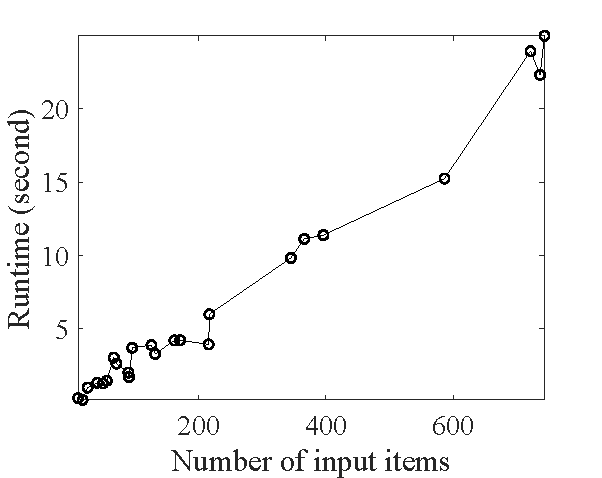
\includegraphics[width=0.45\textwidth]{fig/int-3.pdf}
    \label{items_input}
}
\subfigure{
    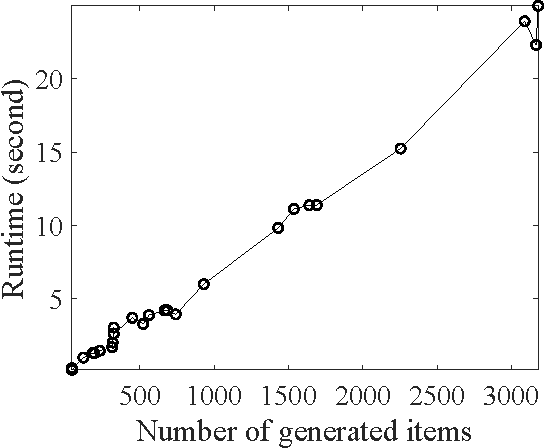
\includegraphics[width=0.45\textwidth]{fig/int-4.pdf}
    \label{items_gen}
}
\caption{(a) Runtime about number of input items; (b) Runtime about number of generated items}
\label{items_all}
\end{figure}

As shown in \reffig{items_input}, the increasement of time is approximately linear about the number of input items. The runtime  in \reffig{items_gen} is more likely  a linear function about the number of generated items. The runtime sometimes decreases due to the remember strategy.

In conclusion, the complexity of our algorithm is exponential about the order of input expression in the worst cases. For the expression with limited orders, the complexity is polynomial about its degree. The complexity is linear when both order and degree are limited. In practice, \texttt{IntCombine} is usually efficient. 

\section{Conclusion} \label{Conclusion-03} 
We have designed a simplification algorithm for arbitrary polynomials of (nested) integrals that might be incomplete matched. The algorithm can handle many cases that cannot be processed by Maple and Mathematica. Furthermore, experiments show that our algorithm is efficient in practice.
